\documentclass[letterpaper,12pt]{article}
\usepackage{amsmath}  % improve math presentation
\usepackage{graphicx} % takes care of graphic including machinery
\usepackage{mathrsfs}


\usepackage[final]{hyperref} % adds hyper links inside the generated pdf file
\hypersetup{
	colorlinks=true,       % false: boxed links; true: colored links
	linkcolor=blue,        % color of internal links
	citecolor=blue,        % color of links to bibliography
	filecolor=magenta,     % color of file links
	urlcolor=blue         
}

\title{Third Assignment for Computational Physics}
\date{\today}
\author{Xinyu Liu}

\begin{document}
\maketitle
\tableofcontents

\section{Problem 1: Computation time for N*N matrice mutiplication}

The associated code of this problem is ps3-1.py.

We do the matrice mutiplication of a N by N matrice. Since we expect that the computation cost is growing with N in a non-linear way, i.e.:

\begin{equation}
    t = \alpha * N^{\beta}
\end{equation}

So, we can test this relationship by doing linear regression against $\ln{t}$ and $ln{N}$, since:

\begin{equation}
    \ln{t} = \ln{\alpha} + \beta * \ln{N}
\end{equation}

In order to reduce the systematic error introduced by computer system, we first try to do linear regression with equally spaced $\ln{N}$ with a broad range of N. The result goes as follows:

\begin{table}[!h]
    \centering
    \caption{The relationship between calculation time(lnt) and matrice size(lnN) with explicit for loop}
    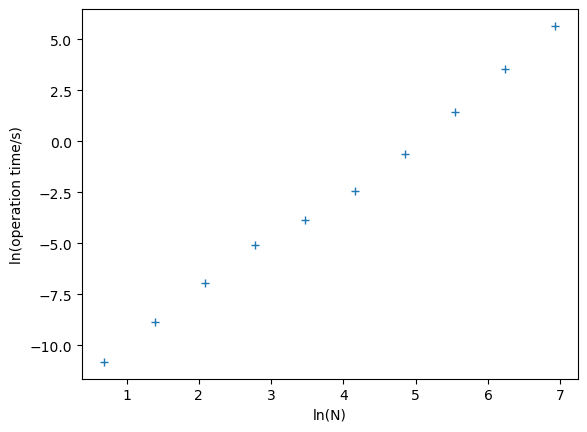
\includegraphics[width=10cm]{ps3-11.png}
    \label{plot}%
\end{table}%

\begin{table}[!h]
    \centering
    \caption{The relationship between calculation time(lnt) and matrice size(lnN) with np.dot method}
    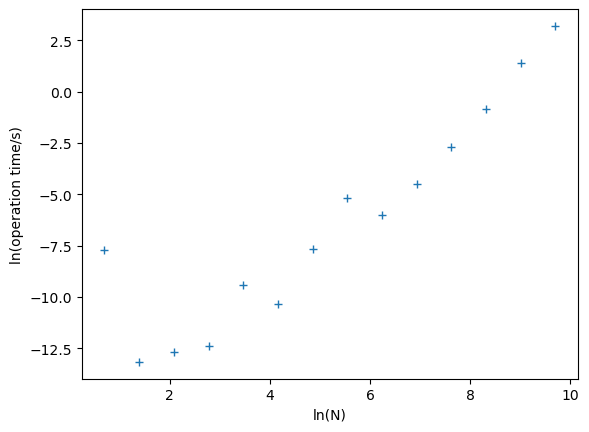
\includegraphics[width=10cm]{ps3-12.png}
    \label{plot}%
\end{table}%
\newpage

We can clearly see that, for smaller size matrice calculation, since the computation is so fast, the time cost depends more on stochastic computer system perturbation and for some random point cost more time than expected. In order to better trace the time dependence of matrice calculation itself, we decide to set N such that the calculation time is always to the order of 1 - 10 seconds. After choosing better N size for each case, we can do similar plotting and linear regression which goes as follows:

\begin{table}[!h]
    \centering
    \caption{The relationship between calculation time(lnt) and matrice size(lnN) with np.dot method}
    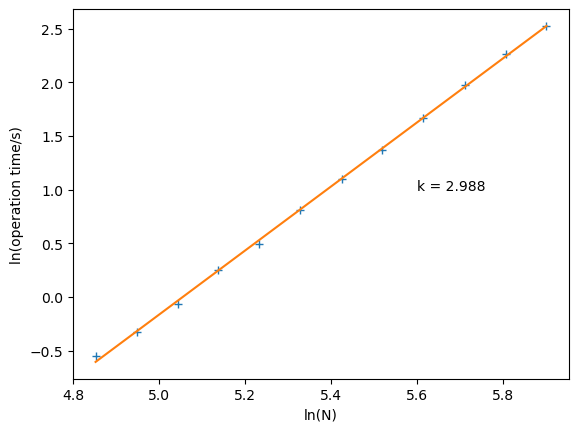
\includegraphics[width=10cm]{ps3-13.png}
    \label{plot}%
\end{table}%

\begin{table}[!h]
    \centering
    \caption{The relationship between calculation time(lnt) and matrice size(lnN) with np.dot method}
    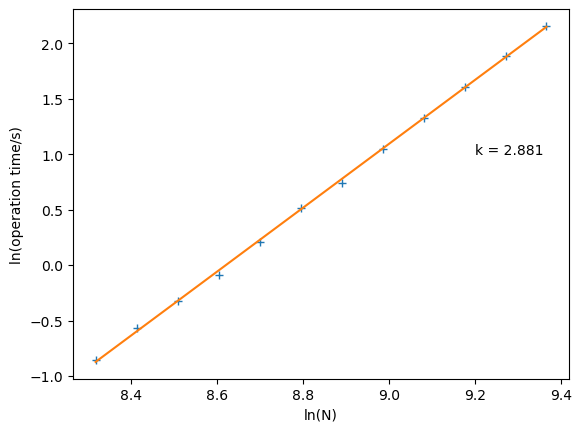
\includegraphics[width=10cm]{ps3-14.png}
    \label{plot}%
\end{table}%

\newpage

We see that after optimizing the choice of N, the linearity between $\ln{N}$ and $\ln{t}$ is clearer. The slope of either case is 2.988 and 2.881, which is close to the expected value of 3. This shows that, for a considerable N(where the calculation time is around the order of seconds), the calculation time approximately grows linearly with $N^3$.

Also, it's evident that the implicit np.dot calculation is much faster than the explicit for loop calculation. The explicit for loop takes more than 200s to calculation the mutiplication of 1000*1000 matrice however for np.dot method it only takes 20s for a 16384*16384 matrice mutiplication. This is because the np.dot method is closer to hardware level and possibly also accelerated by GPU.

\section{Problem 2: Exercise 10.2}

The associated code of this problem is ps3-2.py.

We do the exercise by following the instruction. We use numpy to generate 10000 different random number and compare it with decay possibility at the same time to speed up. This can be seen in our code. The calculation result goes as follows:

\begin{table}[!h]
    \centering
    \caption{The number of different particles under the decay of $^{213}Bi$ in 20000 second}
    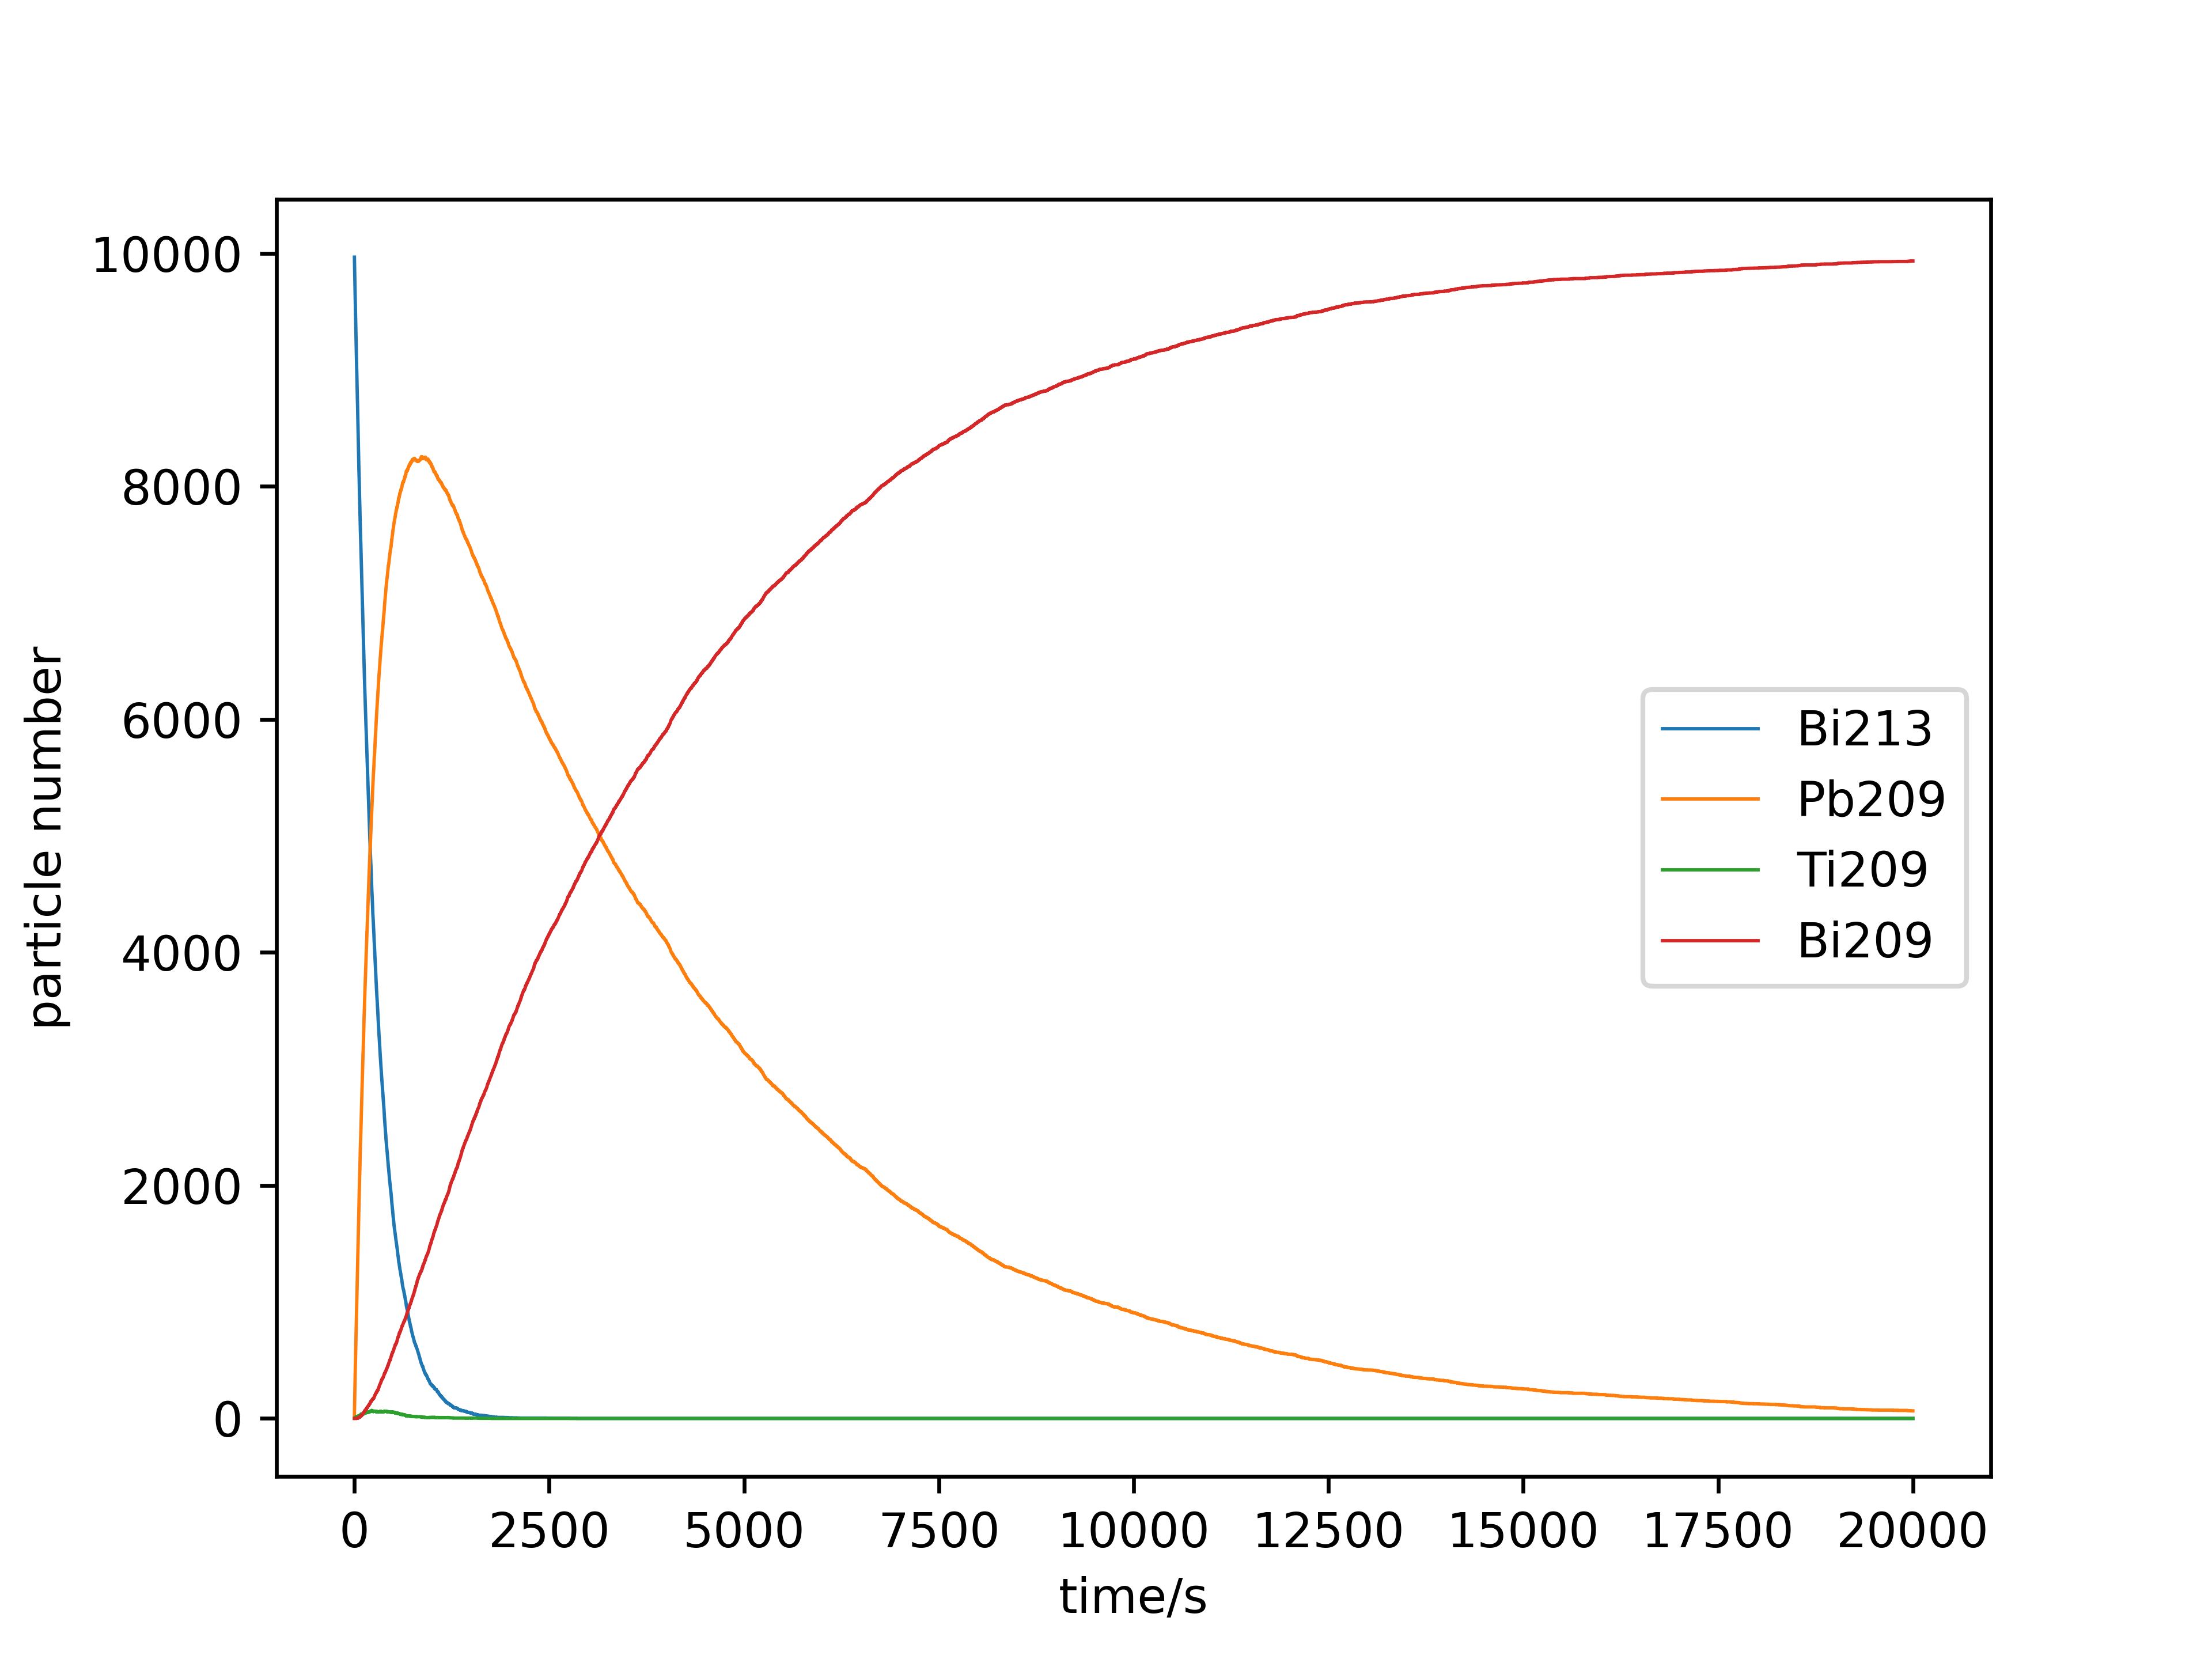
\includegraphics[width=10cm]{ps3-2.png}
    \label{plot}%
\end{table}%


\section{Problem 3: Exercise 10.4}

The associated code of this problem is ps3-3.py.

We do the exercice by following the instruction and generate the variable with correct distribution function of the time a particle decays. In python numpy module we can first generate a random number with even distribution between 0-1(by numpy.random.random())method. We name this stochastic variable z. So the associated PDE for z is:

\begin{equation}
    p(z) = 1
\end{equation}

What we want in our problem is the decay time of a particle t which have the half lifetime $\tau$, whose PDE satisfy:

\begin{equation}
    f(t) = \frac{\ln{2}}{\tau} 2^{-t/\tau}
\end{equation}

So the transfer function between t and z satisfy:

\begin{equation}
    \int_0^{t(x)}  \frac{\ln{2}}{\tau} 2^{-t/\tau} dt = z
\end{equation}

The transfer function is:

\begin{equation}
    t(z) = -\tau \log_2(1-z)
\end{equation}

We can thus generate the decay time by this function and plot a diagram for the number of particle undecayed under certain time.

\begin{table}[!h]
    \centering
    \caption{the number of particle undecayed with time}
    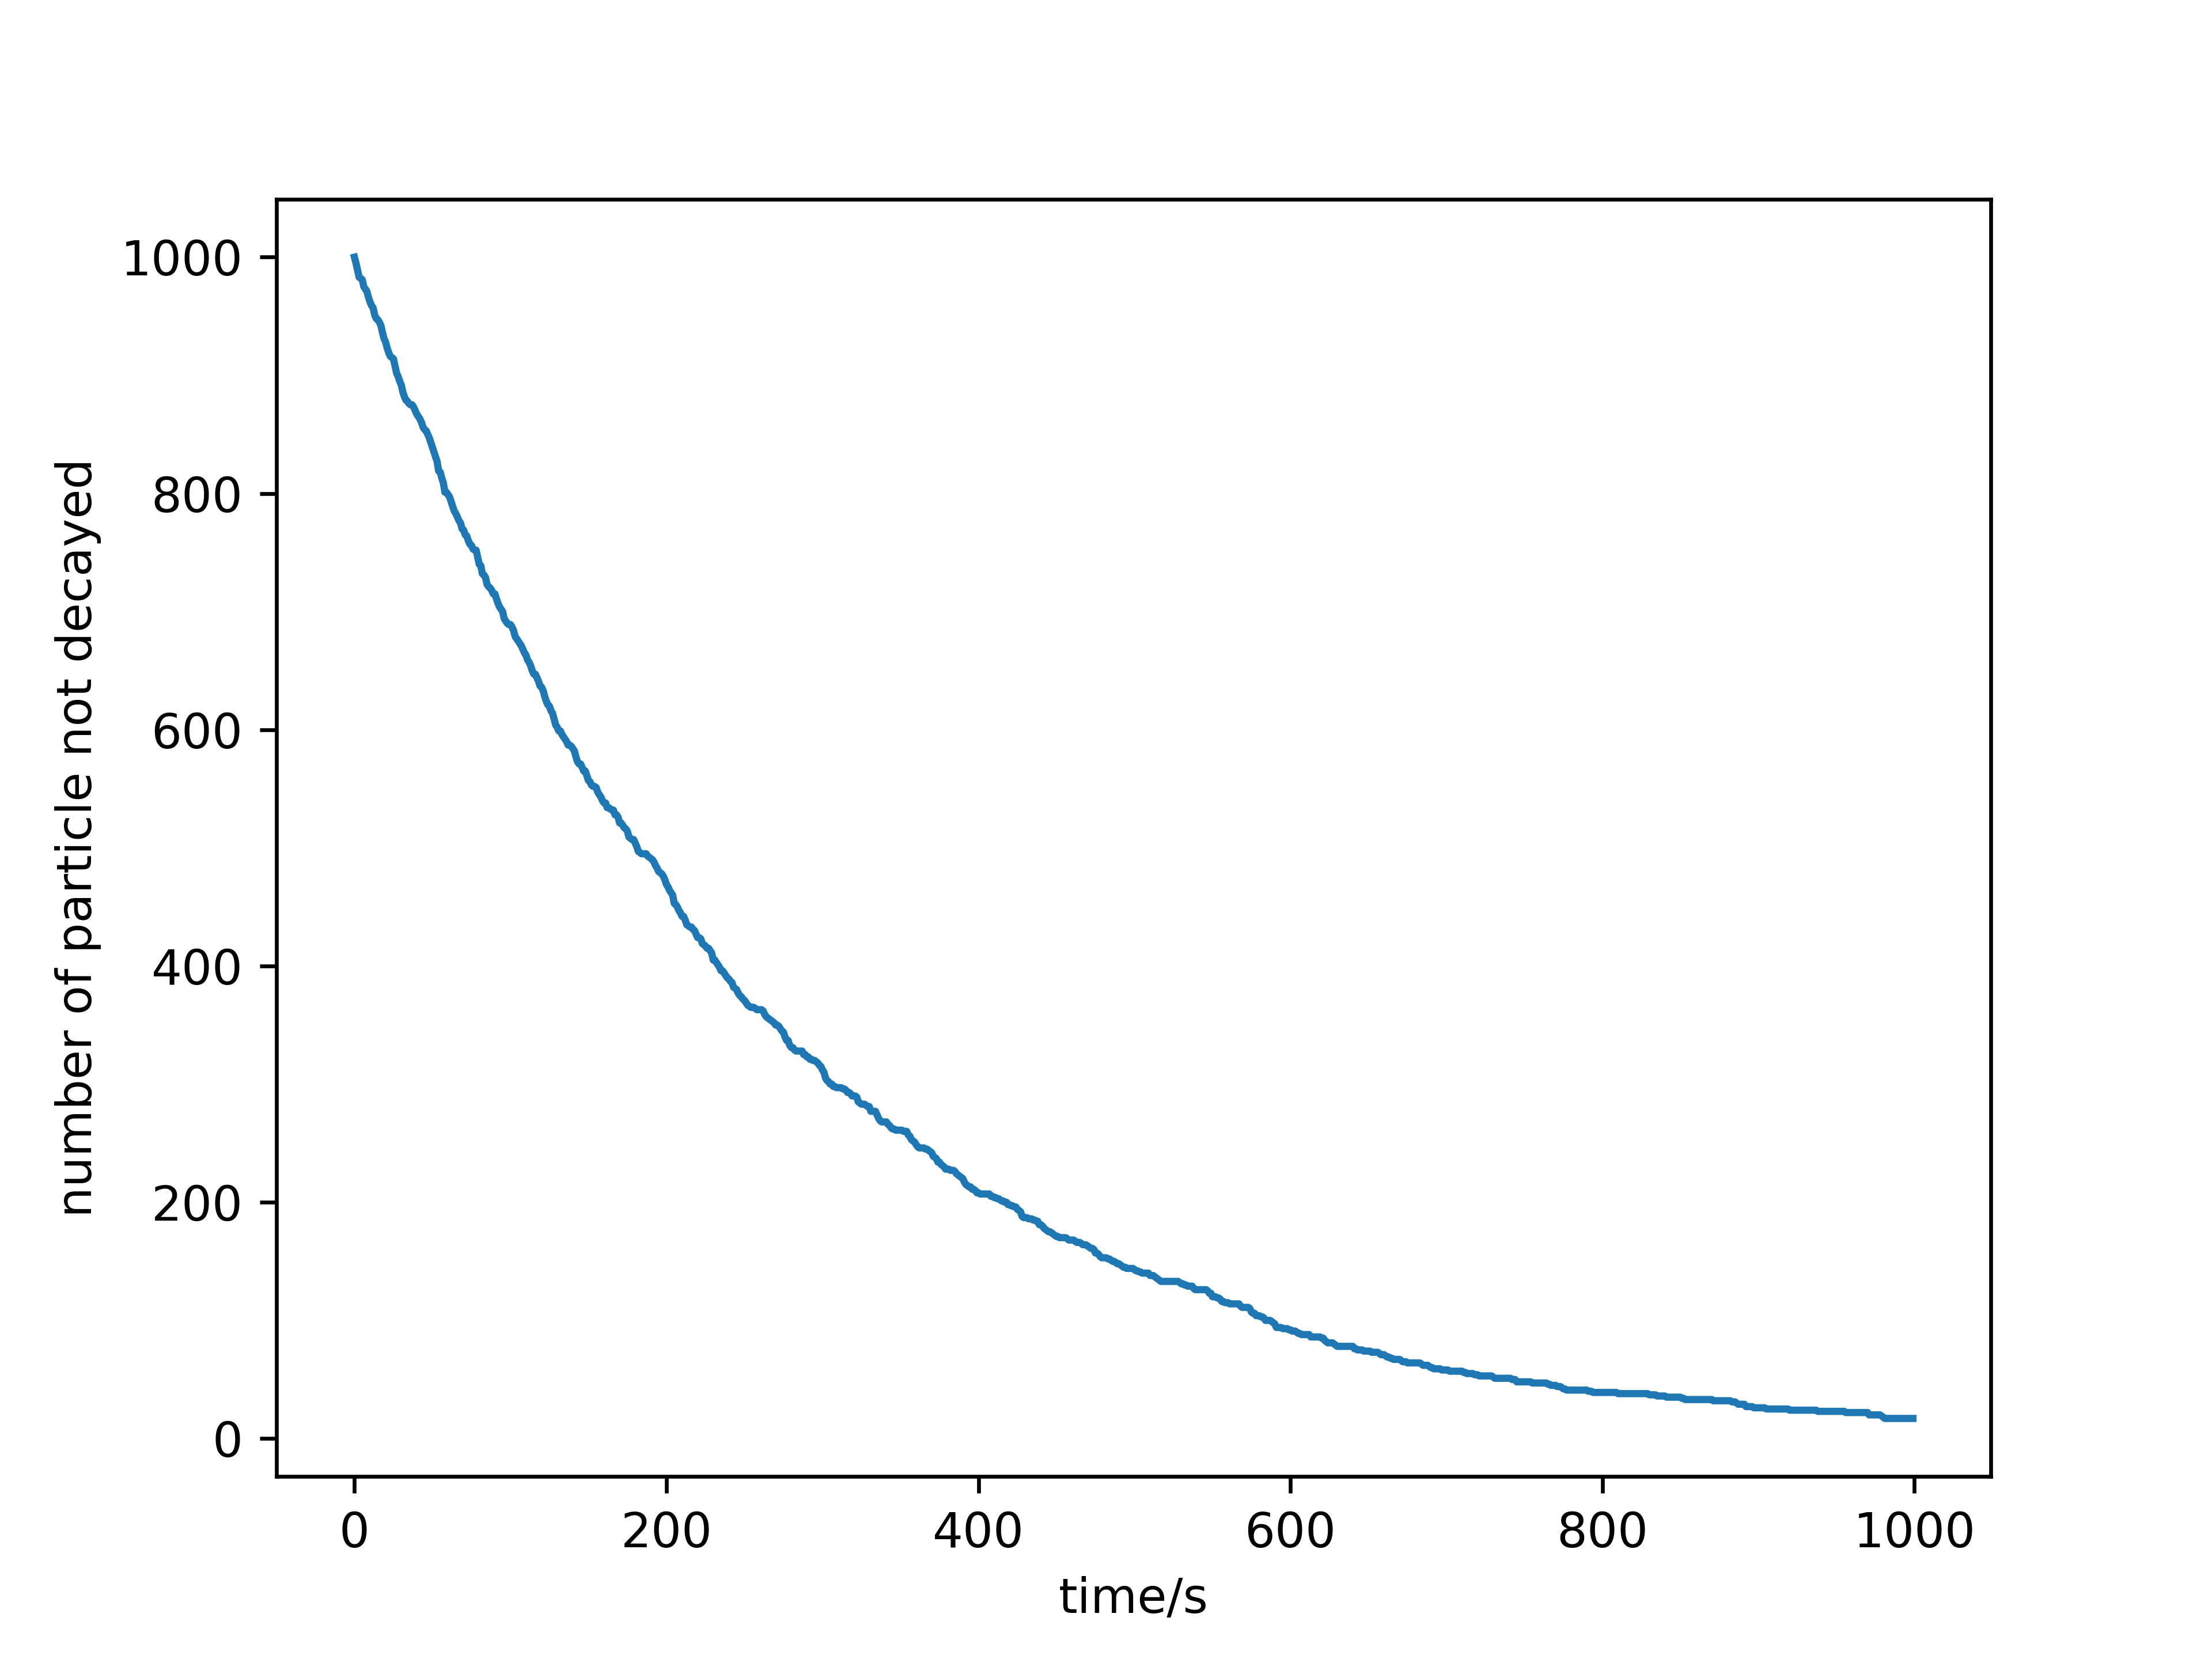
\includegraphics[width=10cm]{ps3-3.png}
    \label{plot}%
\end{table}%

\newpage




\section{Problem 4: Central limit theorem demonstration}

The associated code of this problem is ps3-4.py.

\subsection{Theoretical derivation}

We have N independent variable $x_i$ which each satisfy exponential distribution $p(x_i) = e^{-x_i}$. The variable y is defined as $y = \frac{1}{N}\sum_{i=1}^{N}x_i$. So that the mean value and the variation of y satisfies:

\begin{equation}
    \bar{y} = \overline{\frac{1}{N}\sum_{i=1}^{N}x_i} = \frac{1}{N}\sum_{i=1}^{N}\bar{x_i}
\end{equation}

Since $\bar{x_i} = \int_0^{+\infty} xe^{-x}dx = \Gamma[2] = 1$, where $\Gamma$ represent Gamma function. The mean value of y satisfies:

\begin{equation}
    \bar{y} =\frac{1}{N}\sum_{i=1}^{N}1 = 1
\end{equation}

The variance of y satisfies:

\begin{equation}
    \overline{(\Delta y)^2} =\overline{(\frac{1}{N}\sum_{i=1}^{N}\Delta x_i)^2}
\end{equation}

Since different variable is independen and all variables satisfy same distribution function, the variance of y satisfies:

\begin{equation}
    \overline{(\Delta y)^2} = \frac{1}{N^2}\overline{\sum_{i=1}^{N}(\Delta x_i)^2} = \frac{1}{N} \overline{(\Delta x_1)^2}
\end{equation}

The variance of a single variable can be calculated by:

\begin{equation}
    \overline{(\Delta x_1)^2} = \int_0^{+\infty} (x - 1)^2 e^{-x} dx = \Gamma[3] - 2\Gamma[2] + \Gamma[1] = 2 - 2 + 1 = 1
\end{equation}

So that the variance of y is $\frac{1}{N}$.

\subsection{Computational calculation}

We first generate $10^5$ different y based on $N = 1,10,100,1000$. We draw a histogram to visualize the distribution of $10^5$ different y.

\begin{table}[!h]
    \centering
    \caption{histogram of 100000 y with N = 1}
    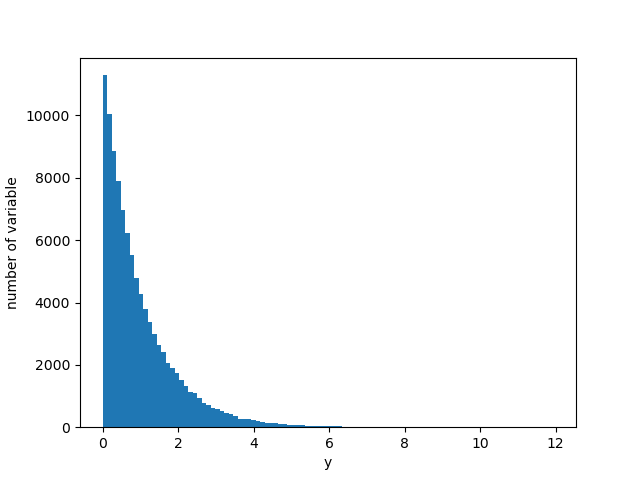
\includegraphics[width=10cm]{ps3-41.png}
    \label{plot1}%
\end{table}%

\begin{table}[!h]
    \centering
    \caption{histogram of 100000 y with N = 10}
    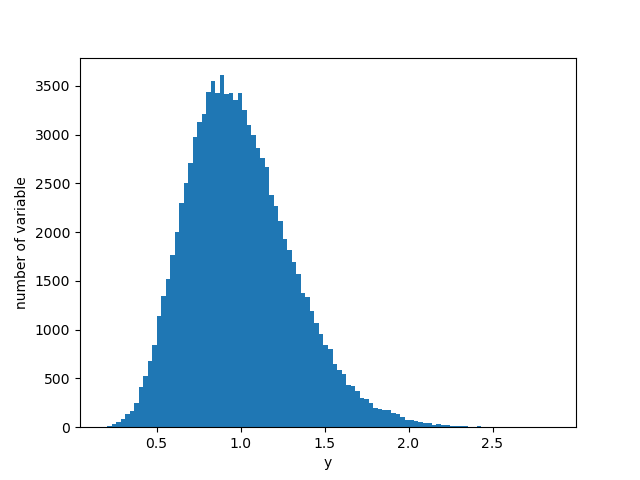
\includegraphics[width=10cm]{ps3-410.png}
    \label{plot10}%
\end{table}%
\newpage

\begin{table}[!h]
    \centering
    \caption{histogram of 100000 y with N = 100}
    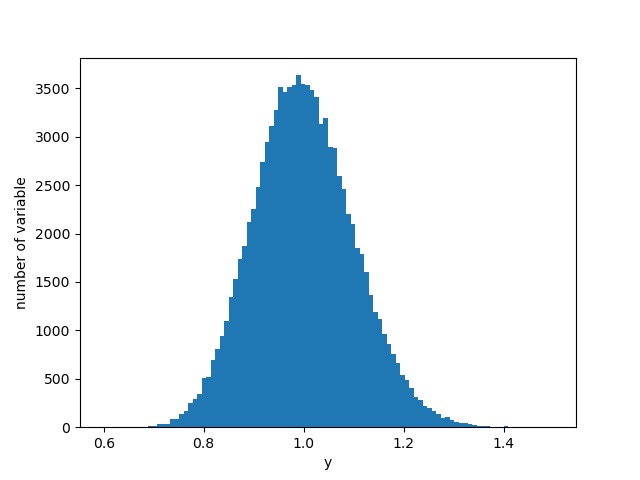
\includegraphics[width=10cm]{ps3-4100.png}
    \label{plot100}%
\end{table}%

\begin{table}[!h]
    \centering
    \caption{histogram of 100000 y with N = 1000}
    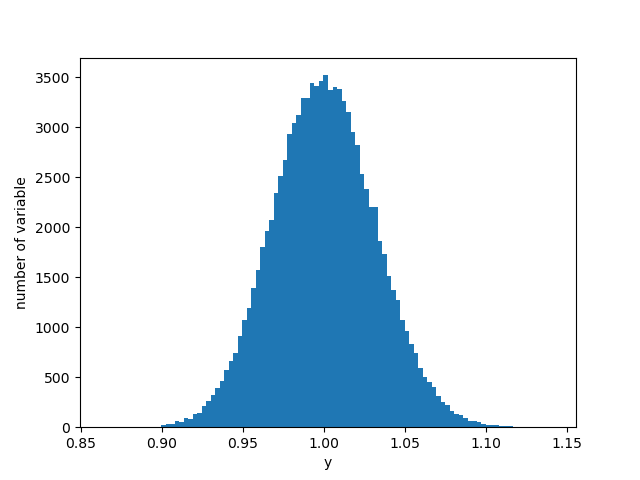
\includegraphics[width=10cm]{ps3-41000.png}
    \label{plot1000}%
\end{table}%

\newpage

\newpage

From these four plots\ref{plot1}\ref{plot10}\ref{plot100}\ref{plot1000}, we can clearly see that the larger the N, the closer the distribution of y is to gaussian. This visualize intuitively how central limit works.

\newpage
We will further try to plot how the mean, variance, skewness, and kurtosis of the distribution change with respected to N. Here's our result:

\begin{table}[!h]
    \centering
    \caption{mean of y w.r.t. N}
    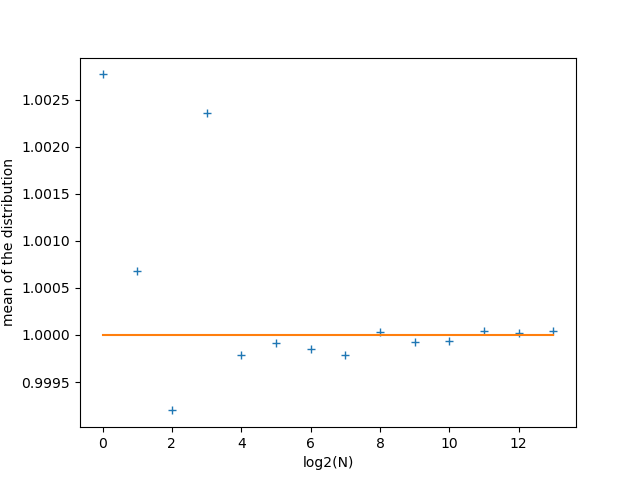
\includegraphics[width=10cm]{ps3-4-21.png}
    \label{plot123}%
\end{table}%
\newpage
Note that in this diagram the orange line represent the theoretical value of mean we've calculated. The result show that our theoretical calculation is correct. The mean is closer and closer to 1 for larger system(large N)

\begin{table}[!h]
    \centering
    \caption{variation of y w.r.t. N}
    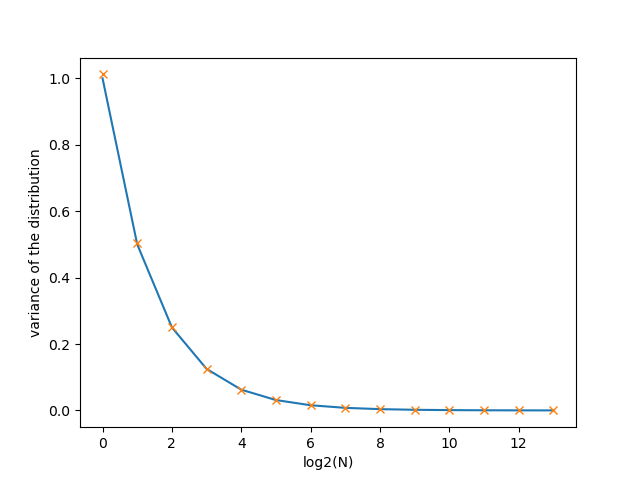
\includegraphics[width=10cm]{ps3-4-22.png}
    \label{plot123}%
\end{table}%
\newpage
Note that in this diagram the blue line represent the theoretical value of variation we've calculated. The result show that our theoretical calculation is correct.
\newpage
\begin{table}[!h]
    \centering
    \caption{skewness of y w.r.t. N}
    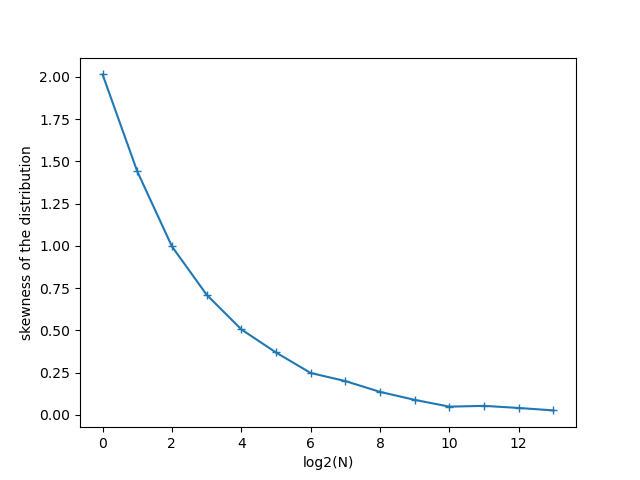
\includegraphics[width=10cm]{ps3-4-23.png}
    \label{plot123}%
\end{table}%

\begin{table}[!h]
    \centering
    \caption{kurtosis of y w.r.t. N}
    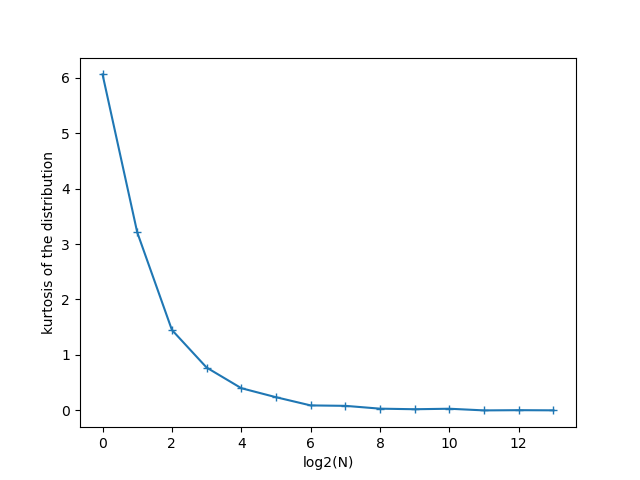
\includegraphics[width=10cm]{ps3-4-24.png}
    \label{plot123}%
\end{table}%

We found that in our calculation, when N equals 8192, the kurtosis of the distribution of y reach 0.01 time the kurtosis of the distribution when N = 1.  when N equals 65536, the skewness of the distribution of y reach 0.01 time the skewness of the distribution when N = 1.  



















\end{document}